\setbeamercolor{background canvas}{bg=fitblue}
\begin{frame}
\frametitle{Textury}
\begin{center}
\Huge {\color{white}Textury}
\end{center}
\end{frame}
\setbeamercolor{background canvas}{bg=white}

\begin{frame}[fragile]
\frametitle{Textury - nahrání rastrových dat}
	\begin{itemize}
	\item Textura je rastrový obrázek, který se namapuje na geometrii.
	\item V OpenGL je to objekt.
\end{itemize}
{\scriptsize
\begin{minted}[bgcolor=bg]{packages/c_cpp.py:CppLexer -x}
//vytvoreni jmena textury
glCreateTextures(GL_TEXTURE_2D,1,&tColor);//vygenerovani jmeno textury pro barvu

//nastaveni parametru textury
//filtering
glTextureParameteri(tColor,GL_TEXTURE_MAG_FILTER,GL_NEAREST);
glTextureParameteri(tColor,GL_TEXTURE_MIN_FILTER,GL_NEAREST);

//wrapping
glTextureParameteri(tColor,GL_TEXTURE_WRAP_S,GL_CLAMP_TO_EDGE);
glTextureParameteri(tColor,GL_TEXTURE_WRAP_T,GL_REPEAT);

//alokace a nahrani dat na GPU
glTextureImage2DEXT(tColor,GL_TEXTURE_2D,0,//alokujeme misto
  GL_RGBA32F,//format ulozeni na GPU (4*float pro pixel)
  WIDTH,HEIGHT,0,GL_RGBA,//format ulozeni dan na CPU
  GL_UNSIGNED_BYTE,//typ dat na CPU
  Data);//data na CPU
\end{minted}
}
\end{frame}

\begin{frame}[fragile]
\frametitle{Nastavení textur}
	\begin{itemize}
	\item V Shader Programu se k nim přistupuje přes uniformní proměnné.
	\item Textura se naváže k texturovací jednotce.
	\item Uniformní proměnná se naváže na texturovací jednotku.
	\end{itemize}
	\begin{figure}[h]
		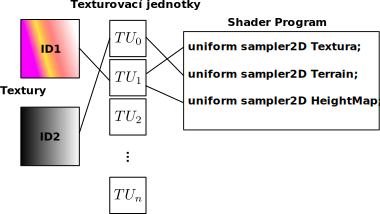
\includegraphics[width=10cm,keepaspectratio]{pics/texture/tu.pdf}
	\end{figure}
\end{frame}

\begin{frame}[fragile]
\frametitle{Nastavení textur}
Shader Program:
{\scriptsize
\begin{minted}[bgcolor=bg]{packages/graphics.py:GLShaderLexer -x}
#version 330
layout(binding=0)uniform sampler2D Textura;
layout(binding=1)uniform sampler2D Terrain;
layout(binding=1)uniform sampler2D HeightMap;
void main(){
  texture(Texture,coords);
  //...
\end{minted}
}
Aplikace:
{\scriptsize
\begin{minted}[bgcolor=bg]{packages/c_cpp.py:CppLexer -x}
//pripojemni textur k texurovacim jednotkam
glBindTextureUnit(0,ID2);
glBindTextureUnit(1,ID1);
\end{minted}
}
\end{frame}

\begin{frame}[fragile]
\frametitle{Adresování textur}
	\begin{itemize}
	\item Textura se adresuje texturovacími koordináty.
	\item Velikost Textury nehraje roli.
	\item Levý dolní roh 2D textury má souřadnice (0.0f,0.0f)
	\item Pravý horní roh 2D textury má souřadnice (1.0f,1.0f)
	\end{itemize}
	\begin{figure}[h]
		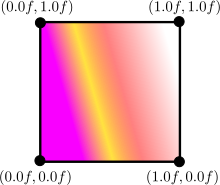
\includegraphics[width=5cm,keepaspectratio]{pics/texture/textura.pdf}
	\end{figure}
\end{frame}

\begin{frame}[fragile]
\frametitle{Atlas textur}
	\begin{itemize}
	\item Více obrázků v jedné textuře.
	\item Staří jedna texturovací jednotka.
	\item Zamezíme přepínání.
	\end{itemize}
	\begin{figure}[h]
		\includegraphics[width=5cm,keepaspectratio]{pics/texture/textureatlas.jpg}
	\end{figure}
	\url{http://www.scriptspot.com/3ds-max/scripts/texture-atlas-generator}
\end{frame}

